\documentclass[12pt]{article}
\usepackage[parfill]{parskip}
\usepackage{amsmath}
\usepackage{amssymb}
\usepackage{bm}
\usepackage{enumerate}
\usepackage{fancyvrb}
\usepackage[top=1in, bottom=1in, left=1in, right=1in]{geometry}
\usepackage{hyperref}
\hypersetup{
	colorlinks=true,
}
\usepackage{placeins}
\usepackage{tikz}
\usepackage{tikzsymbols}
\usepackage{todonotes}
\usepackage{bbm}
\usepackage{color}
\usepackage{enumitem}
\usepackage{xcolor}
\newcommand{\rmn}[1]{{\textcolor{blue}{\bf [{\sc rmn:} #1]}}}
\DeclareMathOperator*{\argmax}{arg\,max}
\usepackage{algorithmicx}
\usepackage{algorithm}
\usepackage{algpseudocode}
\usepackage{multirow}
\usepackage{rotating}

\usetikzlibrary{positioning,calc}
%%%%%%%%%
\usepackage[most]{tcolorbox}
\newtcolorbox[]{solution}[1][]{%
	breakable,
	enhanced,
	colback=white,
	title=Solution,
	#1
}
%%%%%%%%%%
\title{10-703 Deep Reinforcement Learning and Control\\
	Assignment 3\\
	Fall 2018 \\  
}
\author{ielshar \\ mharding}
\date{October 26, 2018}
\begin{document}
	
	\maketitle
	
	\section*{Problem 1: Reinforce}
	\begin{enumerate}
		\item  Describe your implementation:
		\begin{itemize}
			\item Neural Network Architecture:  same as given in JSON file.
			\item Learning rate: 0.001
			\item Discount factor $\gamma: 1$
		\end{itemize}
		\item 
		\begin{figure}[H]
			\begin{center} 
				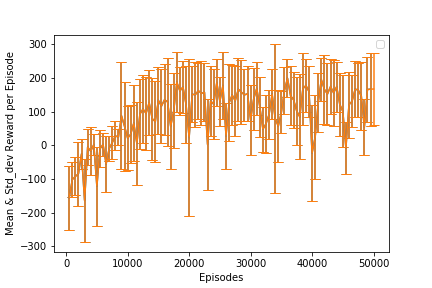
\includegraphics[scale=.73]{figures/Reinforce_LC_50.png}
			\end{center}
			\caption{Reinforce Algorithm: learning curve - Every k=500 episodes the current policy is tested on 100 episodes. The plot shows the mean and standard deviation of each of this tests.  } 	\label{1}%
		\end{figure}
	\end{enumerate}
	
	Figure \ref{1} above shows that our agent was able to achieve a mean reward of 200  or slightly more or less at several points (after 36000, 41500 episodes) through out the training. Since no baseline was used in our Reinforce algorithm one can see that the test results have a high variance. This is somehow expected though as the total return at the end of episode varies highly from one episode to another.
	
	\section*{Problem 2: Advantage-Actor Critic}
	\begin{enumerate}
		\item Implementation details:
		% Table generated by Excel2LaTeX from sheet 'Sheet2'
		\begin{table}[H]
			\centering
			\caption{A2C Implementation}
			\begin{tabular}{|c|p{11.085em}|l|}
				\hline
				\multicolumn{3}{|c|}{A2C } \\
				\hline
				N     & Settings & \multicolumn{1}{p{16em}|}{value} \\
				\hline
				\multirow{4}[8]{*}{1} & Actor NN Architecture  & \multicolumn{1}{p{16em}|}{Same as given in JSON file} \\
				\cline{2-3}          & Critiic NN Architecture  & \multicolumn{1}{p{16em}|}{MLP with 3 layers each with 30 hidden units and relu activation} \\
				\cline{2-3}          & Actor learning rate & 0.001 \\
				\cline{2-3}          & Critic learning rate & 0.001 \\
				\hline
				\multirow{4}[8]{*}{20} & Actor NN Architecture  & \multicolumn{1}{p{16em}|}{Same as given in JSON file} \\
				\cline{2-3}          & Critiic NN Architecture  & \multicolumn{1}{p{16em}|}{MLP with 3 layers each with 20 hidden units and relu activation} \\
				\cline{2-3}          & Actor learning rate & 0.001 \\
				\cline{2-3}          & Critic learning rate & 0.001 \\
				\hline
				\multirow{4}[8]{*}{50} & Actor NN Architecture  & \multicolumn{1}{p{16em}|}{Same as given in JSON file} \\
				\cline{2-3}          & Critiic NN Architecture  & \multicolumn{1}{p{16em}|}{MLP with 3 layers each with 20 hidden units and relu activation} \\
				\cline{2-3}          & Actor learning rate & 0.001 \\
				\cline{2-3}          & Critic learning rate & 0.001 \\
				\hline
				\multirow{4}[7]{*}{100} & Actor NN Architecture  & \multicolumn{1}{p{16em}|}{Same as given in JSON file} \\
				\cline{2-3}          & Critiic NN Architecture  & \multicolumn{1}{p{16em}|}{MLP with 3 layers each with 20 hidden units and relu activation} \\
				\cline{2-3}          & Actor learning rate & 0.0008 \\
				\cline{2-3}          & Critic learning rate & 0.001 \\
				\hline
			\end{tabular}%
			\label{table}%
		\end{table}%
	* discount factor was set to 1 in all implementations.
	\newpage
		\item  Plots:
		\begin{itemize}
			\item N=1 :  First reached a mean reward of 225 after 20500 episodes.
			\begin{figure}[H]
				\begin{center} 
					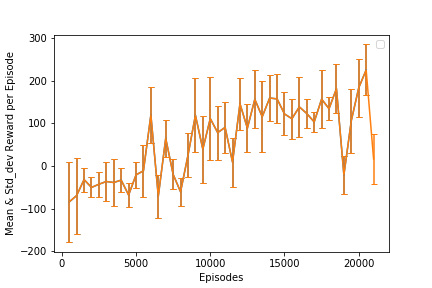
\includegraphics[scale=.73]{figures/A2C_LC_N=1_21.png}
				\end{center}
				\caption{A2C Algorithm N=1: learning curve - Every k=500 episodes the current policy is tested on 100 episodes. The plot shows the mean and standard deviation of each of this tests.  } 	\label{2}%
			\end{figure}			
			\item  N=20 :   First reached a mean reward of 200 after 6500 episodes.
			\begin{figure}[H]
				\begin{center} 
					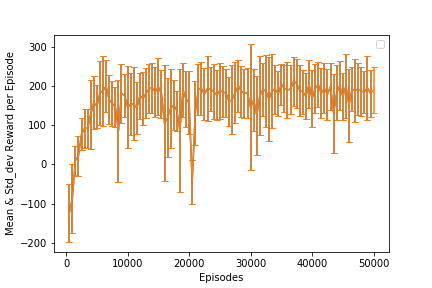
\includegraphics[scale=.73]{figures/A2C_LC_N=20_50.png}
				\end{center}
				\caption{A2C Algorithm N=20: learning curve - Every k=500 episodes the current policy is tested on 100 episodes. The plot shows the mean and standard deviation of each of this tests.  } 	\label{3}%
			\end{figure}
			\item N=50:   First reached a mean reward of 201 after 20500 episodes.
			\begin{figure}[H]
				\begin{center} 
					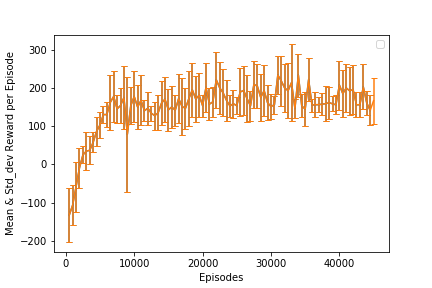
\includegraphics[scale=.73]{figures/A2C_LC_N=50_45.png}
				\end{center}
				\caption{A2C Algorithm N=50: learning curve - Every k=500 episodes the current policy is tested on 100 episodes. The plot shows the mean and standard deviation of each of this tests.  } 	\label{4}%
			\end{figure}
			\item N=100 actor lr=0.0008 and critic lr=0.001 :  First reached a mean reward of 200 after 25500 episodes.
			\begin{figure}[H]
				\begin{center} 
					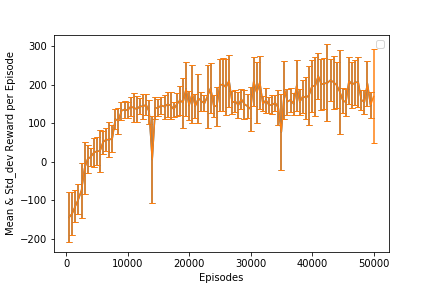
\includegraphics[scale=.73]{figures/A2C_LC_N=100_50.png}
				\end{center}
				\caption{A2C Algorithm N=100: learning curve - Every k=500 episodes the current policy is tested on 100 episodes. The plot shows the mean and standard deviation of each of this tests.  } 	\label{5}%
			\end{figure}	
					\item N=100 actor lr=0.001 and critic lr=0.001 : First reached a mean reward of 204 after 32000 episodes.
			\begin{figure}[H]
				\begin{center} 
					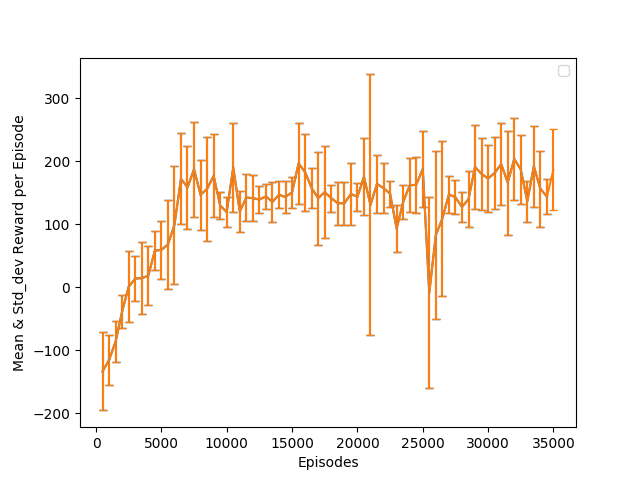
\includegraphics[scale=.73]{figures/A2C_LC_N=100_35.png}
				\end{center}
				\caption{A2C Algorithm N=100: learning curve - Every k=500 episodes the current policy is tested on 100 episodes. The plot shows the mean and standard deviation of each of this tests.  } 	\label{6}%
			\end{figure}	  
		\end{itemize}
		
		\item  Reinforce and A2C comparisons:\\
		Compared to Reinforce, n-steps A2Cs have much lower variance and accelerated learning expect for the case when n=1. This is mainly due the added effect of the critic which bootstraps unlike the Reinforce algorithm with uses the MC return that has high variance. The case of A2C with one-step look critic introduce much more bias than n=20,50 and 100 A2Cs that is why it's much harder to learn.
		It seems that A2C algorithm with n=20, 50 and 100 learn faster than all the others. Even though we were able to achieve a better performance for n=100 with an actor learning rate  of 0.0008 as seen in Figure \ref{5} above, we run A2C n=100 again for 35000 episodes with an actor lr=0.001 (Figure \ref{6} ) which is the same as the one used for A2C n=20 and n=50. This is done to make sure the comparison regarding speed of learning is fair enough since now the only difference between them is n, the number of steps. (Note that we fix the random seed in all of the implementations). 
		
		A2C n=20 was the fastest to reach a mean reward of 200 or greater. It achieved that after only 6500 episodes.
		A2C n=50 (50-steps return) comes second with 20500 episodes.  
		Third comes A2C n=100 with 32000 episodes. 
		Fourth comes Reinforce with 36000 episodes. 
		A2C n=1 was not able to achieve 200 with the same neural architecture for the critic as the other algorithms. However using a critic NN architecture that include 3 layers each with 30 units this time A2C n=1 achieved a reward of 225 after 20500 episodes similar to A2C n=50.
		Comparing figures \ref{3}, \ref{4} and \ref{6},
		it can be seen that A2C n=20 has the steepest rate of learning then comes n=50 and finally n=100. 
		We believe this is the case since 20-step and 50-step A2Cs have the best balance between bootstrapping using the value function and using the full MC return.
		
		
		
		
	\end{enumerate}
	
	
	
	
\end{document}